\subsection{Ambiguity-Band Stopping Policies}
\label{app:ambiguity_bands}

The \gls{method} procedure is agnostic to the form of the stopping policy $D_\lambda$, provided that the policy family is fixed prior to calibration and yields a bounded trajectory-level loss. In practice, however, the efficiency of safe stopping depends strongly on how this policy family is parameterized. We therefore instantiate $D_\lambda$ using a family of \emph{ambiguity-band stopping rules} defined over time-dependent predictive scores. This construction is used primarily for the MRI experiments, where clinically relevant false negative and false positive tradeoffs make thresholded score bands a natural decision primitive.

\paragraph{Predictive scores.}
Suppose that at acquisition time $t\in\{0,\dots,T-1\}$, the model outputs a positive-class score $S_{i,t,k}\in[0,1]$ for sample $i$ and label $k$, based on the cumulative partial observation $X_i^t$. In the multi-task setting, $k\in\{1,\dots,K\}$. Larger values of $S_{i,t,k}$ indicate stronger evidence for the positive class.

\paragraph{Baseline ambiguity anchors.}
For each acquisition step $t$ and task $k$, we define a pair of nominal ambiguity anchors $b^-_{t,k}, b^+_{t,k}$, with $0\le b^-_{t,k}\le b^+_{t,k}\le 1$, that identify a region of the score space where the model is considered ambiguous. Intuitively, scores below $b^-_{t,k}$ provide evidence for a negative decision, while scores above $b^+_{t,k}$ provide evidence for a positive decision. The interval $[b^-_{t,k},\, b^+_{t,k}]$ therefore serves as a time-specific uncertainty band. In our experiments, these anchors are estimated from a small held-out estimation set by comparing the empirical score distributions of positive and negative examples at each acquisition step. Concretely, for a fixed $(t,k)$, let
\begin{align*}
S^+_{t,k}=\{S_{i,t,k}: y_{i,k}=1\},
\qquad
S^-_{t,k}=\{S_{i,t,k}: y_{i,k}=0\},
\end{align*}
denote the positive- and negative-class score collections. We then define the nominal ambiguity anchors as the narrowest non-inverted quantile bracket within a pre-specified quantile family, yielding a data-driven aggressive endpoint for the band family. Importantly, these anchors are not themselves claimed to be risk-calibrated; rather, they serve to define an ordered family of stopping policies, while the actual statistical guarantee is supplied downstream by the \gls{method} calibration procedure.

\paragraph{Band modulation by $\lambda$}
Given the nominal anchors $(b^-_{t,k}, b^+_{t,k})$, we define a one-parameter family of effective ambiguity bands indexed by $\lambda\in[0,1]$:
\begin{align}
\label{eq:sym_bands_main}
\ell_{t,k}(\lambda)=\lambda\, b^-_{t,k},
\qquad
u_{t,k}(\lambda)=\lambda\, b^+_{t,k} + (1-\lambda).
\end{align}
This construction interpolates between:
\begin{itemize}
    \item \textbf{maximal ambiguity} at $\lambda=0$, where $[\ell_{t,k}(\lambda),u_{t,k}(\lambda)]=[0,1]$, and
    \item the \textbf{nominal ambiguity band} at $\lambda=1$, where $[\ell_{t,k}(\lambda),u_{t,k}(\lambda)]=[b^-_{t,k},b^+_{t,k}]$
\end{itemize}
Larger values of $\lambda$ therefore correspond to narrower ambiguity bands and more aggressive stopping rules.


\paragraph{Stopping rule.}
For a fixed $\lambda$, the stopping rule halts acquisition at the first time all tasks simultaneously exit their ambiguity bands. Formally, define the stopping time
\begin{align*}
\tau_\lambda(X_i) &= \inf\left\{t\in\{0,\dots,T-1\}: \forall k,\;
                    S_{i,t,k}\notin [\ell_{t,k}(\lambda),u_{t,k}(\lambda)]\right\}
\end{align*}
If no such time exists, we set $\tau_\lambda(X_i)=\infty$ and allow the policy to abstain or defer to the terminal horizon, depending on the risk formulation under consideration.

\paragraph{Terminal prediction.}
The ambiguity band jointly determines both stopping and prediction. Acquisition continues while the score remains inside the effective ambiguity interval \([\ell_{tk}(\lambda),u_{tk}(\lambda)]\). Once the score exits this interval, the side of exit determines the terminal class label: scores below the lower boundary are assigned to the negative class, while scores above the upper boundary are assigned to the positive class. Thus, for a single task, the sequential policy is
\[
D_\lambda(X^t)=
\begin{cases}
0, & S_t(X^t)<\ell_t(\lambda),\\
1, & S_t(X^t)>u_t(\lambda),\\
\mathrm{CONTINUE}, & S_t(X^t)\in[\ell_t(\lambda),u_t(\lambda)].
\end{cases}
\]
In the multi-task setting, acquisition halts once every task has exited its corresponding ambiguity band, and the terminal label for each task is determined by the side on which its score exits. This yields a complete stopping-and-prediction policy $D_\lambda$, which can then be certified by the procedure in Section~\ref{sec:rcs}.

\paragraph{Interpretation.}
The ambiguity-band construction should be viewed as a practical policy-family parameterization rather than as the source of the final guarantee. The role of the nominal anchors is to define an aggressive score-space ambiguity template at each acquisition time, and the role of $\lambda$ is to control how aggressively that ambiguity region is shrunk. The final risk guarantee is not inherited from the bands themselves, but from the downstream calibration procedure applied to the resulting trajectory-level stopping policies.

\newpage
\subsection{Clinical Prostate MRI Acquisition States}
\begin{figure}[h]
\centering
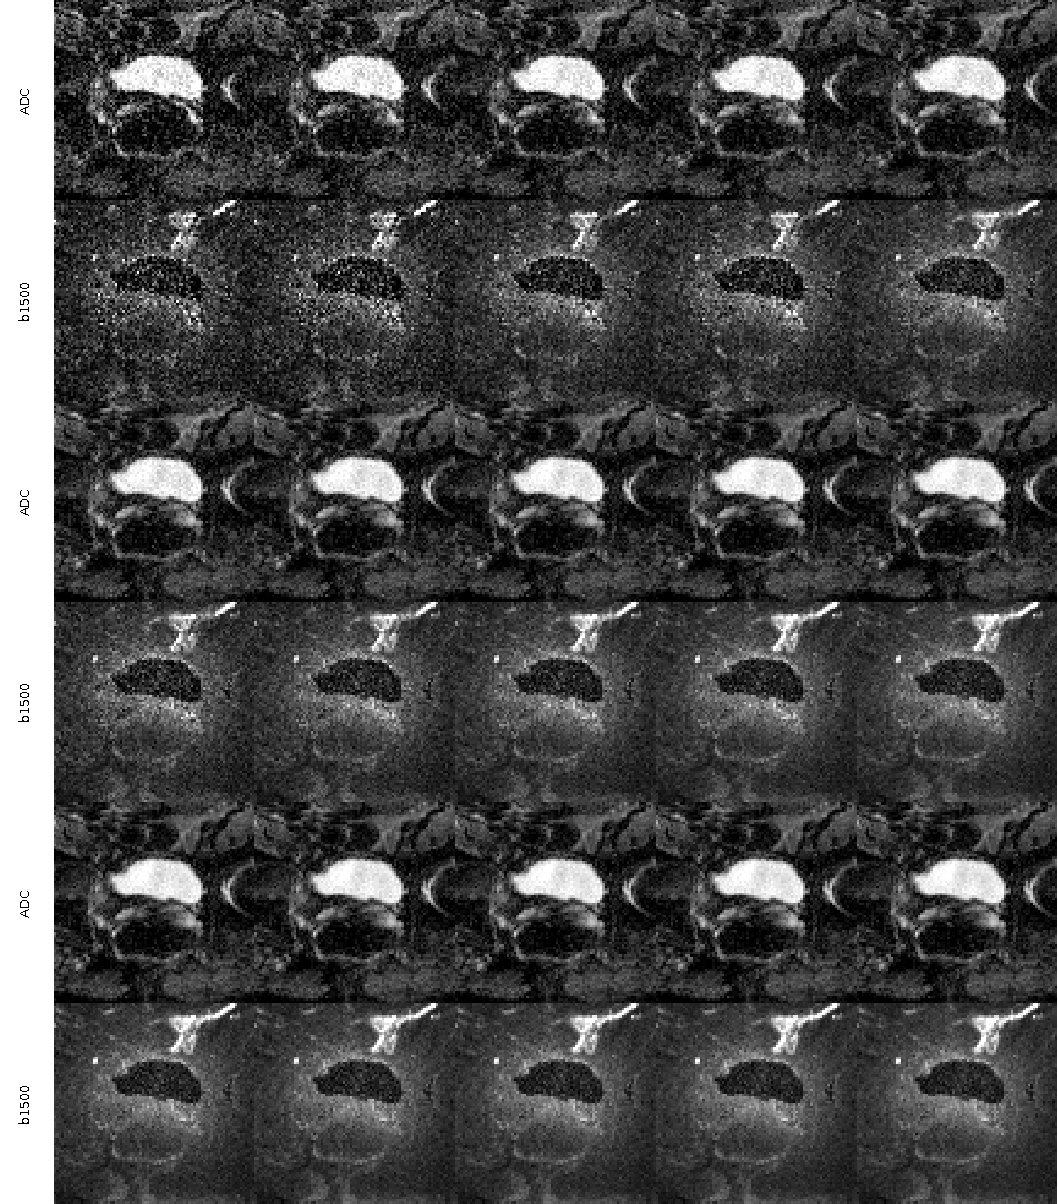
\includegraphics[width=\linewidth]{figures/prostate_dwi_acquisition_states_15.pdf}
\caption{Prostate DWI-derived images across sequential acquisition states.
Each tile shows ADC above computed high-b-value DWI ($b=1500$) for the same scan and slice.
Tiles are ordered left-to-right and top-to-bottom according to scanner acquisition order, from $1/1$ to $4/12$ acquired $b=50$/$b=1000$ averages.
}
\label{fig:prostate_dwi_acquisition_states}
\end{figure}